\documentclass[11pt]{article}
\usepackage{fullpage}
\usepackage{graphicx}
\title{Dream User Interface for Web Browsing}
\author{Miguel Vazquez}
\begin{document}
\maketitle
\tableofcontents

\section{Introduction}
Web browsers are a tool that many of us are used to nowadays. However that is not to say that this tool has reached its pinnacle of perfection and it does not mean that it is not what the people need. It should also be mentioned that this is still a tool that can only be used to its maximum potential by a select group of people. This in itself is good except that the select few who use it well have had teachings with it and does not allow for other to do so effectively. 
% JD: Not sure what you mean by "have had teachings" with a web browser.

\section{Components}
There are various ideas that I have related to a user interface for web browsing. They are as follows.

\subsection{Working with Bricks}
Whether a person is young or old they never lose the fascination of building something. The ability to create and then use something can be cause for a grand feeling of accomplishment that can cause for a desire to create even more. This feeling of creation is something that makes Legos so popular and is something that is felt whenever one uses them. My idea for this is to allow for simple piecing together and taking apart of various aspects related to the browser. The browser would have different media squares or “bricks.” These would be attachable to anything within the browser and can come in various sizes and uses. The idea is that each of these bricks can act as a browser. By putting multiple bricks together one can view multiple pages at once. Of course this may not cause the most comfort for the user, and each media square can be made larger so as to take an entire monitor. This is partially done to improve on the idea of tabs. They are very helpful tools but at times one may have multiple tabs from the same website causing them all to have the same name. This causes the possibility that a user will need to go through some trial and error in order to find the tab they want. The ability to have a window to each individual tab will cause this problem to go away. The next aspect to this brick idea is that a user can combine the bricks to make the screen bigger. This allows for a user to make a video play on a screen they specifically want. The inclusion of color to each brick also allows for some added color to what can sometimes be considered as a drab and boring user experience. The hope is that with this customizability, the user will be excited to be using their browser even if it isn’t for the sites they will access or the media they will find.
% JD: This is a very interesting idea.  Now, although I think I can visualize what
%     you mean here, it would have been even better if you had sketched something
%     up, no matter how rough, to better communicate what you mean.
%
%     Also, watch out when writing in Word first then changing to LaTeX.  Your quotes
%     and apostrophes (e.g., "bricks" and isn't) are the curly kind, which LaTeX does
%     not acknowledge.

\subsection{Achievement System}
Something that has been appearing more and more with interactive media, namely video games is a system of achievements. Although these systems don’t actually mean anything outside of the media they are found in they do have certain desirability. The achievements or badges can be related to a person’s specific account. The thing about these achievements is that they will be directly related to the usage of the web browser. They will be challenges such as linking bricks in a certain matter or using certain properties of the bricks. However some more challenging achievements will also be made available. The trick to these achievements is that they will have tips and tricks related to them as well as forums for the users to help one another. These trickier achievements will include adding new functionality to the bricks, inspecting the elements of a webpage, and even creating simple HTML webpages. By “challenging,” it is obvious that it refers to anything related to programming and background elements at play that provide the user with the browsing experience they enjoy. One of the achievements will aimed towards showing the user how to submit any of their ideas or code that they believe should be shared. Of course their own creations can be used by themselves freely, but by submitting their work the people in charge of the browser can choose what should be added. The work can also be submitted to the forums so that the users themselves can vote over which user created features they would like to use freely. This will allow for an interesting interaction between company and users. It is basically all meant with the users in mind.
% JD: This is also an interesting idea, but begins to cross the line between a
%     user interface element and a feature.  The idea of achievements, in itself,
%     is very much a feature ("utility" vs. "usability").  The achievements would
%     have to be used, and presented, in a very particular way so that they are
%     more closely bound to interaction design than as an interesting web browser
%     feature.  The way you describe it, it's sort of in-between.  It is definitely
%     new functionality, but as a way to encourage the user to explore the browser
%     or learn new tasks, it intersects with interaction design also.
%
%     Again, going beyond words and trying to illustrate your concept would go a
%     long way toward refining this idea to a genuine user interface innovation.

\subsection{Improved User Experience}
% JD: The motivation behind the wait-time idea is appreciated, but this does have
%     genuine practical considerations---specifically, that there really are times
%     when the system simply doesn't know how long a connection will take to finish.
%     It can make guesses based on prior history, but at any given moment that guess
%     can be very wrong.  This then becomes a point of diminishing returns---how
%     much of the computing resource are you willing to devote to filling in the
%     user's wait time, which may be unpredictable?
Besides the brick idea that has already been mentioned there are a couple more ideas that can easily make the web browsing experience even more enjoyable. One such idea is meant for the loading of the different web pages. This wait time can feel tiresome for people and can often be one of the most difficult and annoying points of the web browsing experience. The idea for this to be fixed is to have the browser know internet speed, and the size of the information that needs to be received for the site. With this in mind an exact time for loading could be made. As was stated the waiting can be the worst part and not knowing how long one has to wait can make it even worse. The idea is that by telling the user how much time it will take, they can do other things to pass their time instead of sitting there. An idea that goes along with this timer is the inclusion a time passing application. This could be a variety of things such as a game, a memo pad, or even something else that the user has created. This will help the user as it will make the wait time for the load feel less tedious, and also keep the user on the web browser, so that they do not do something else on their computer that could stray them away from the reason they opened their web browser in the first place. This can help cause a more enjoyable experience for the user. Another feature that this browser will have is the ability of auto-scrolling to allow the user to read without having to interact with the brick themselves. This feature can be activated through the menu system that will appear on every brick as a sort of home page or through keyboard shortcuts. The final part of this enhanced experience leans towards the safety of the user. This involves changing the mouse cursor to an arrow with a question mark, or some other symbol like that which will clearly tell the user that they should be cautious with the object they plan on selecting. This would also involve asking the user a second time whether they want to have a toolbar attached to the web browser. It is no secret that nowadays most downloads mention that they have a toolbar from their company that they now offer to the user for their browsing experience. Many people download what they need and download the toolbars along with it whether it is because they think it will be a good idea, or do not pay attention to what is being downloaded. The second check for the toolbar will show the user what is being offered once more but also show how the performance of the browser will be affected. This means that the speed of the browser, as well the capacities of the browser will be mentioned. These statistics will be listed in a simplified manner that the user can actually understand it. This will allow the user to become familiar with the terminology related to computers and interest them in efficiency of the browsing experience and their own programs. 
% JD: The other ideas in this paragraph have similar give/take tradeoffs too.
%     Autoscrolling is interesting, but needs more detail (an illustration would
%     be nice here, again).  User safety is another one of those "it works if
%     your information is known or reliable" things, like the wait time issue.
%     Under what criteria should the user use caution?  Do different users have
%     different levels of caution?  At what point will the warnings become annoying
%     instead of helpful?  The breadth of ideas is nice, but it also looks like
%     the sheer number of them has kept your from exploring them more deeply.

\section{Scenarios}


\subsection{Media Viewing while working}
The media bricks are meant to allow the user a lot of mobility and the ability to view the internet as they please. The bricks are meant to make it easier to resize a window for the comfort of the user. Although people do have the ability to click and drag on a corner the ability to add a preset size can add for a bit more comfort and entertainment. By combining the squares one can make a video play in whatever size or shape that they please. This allows for the user to make a perfectly sized video screen for them to continue working. These windows also allow for a video viewing experience that does not require seeing the rest of the web site and because the bricks are an entire tab there is nothing to distract the viewer from the video. Figure ~\ref{YouWork} shows a current format for video watching and working. Figure  ~\ref{YouWorkClean}  more or less shows the type of view the brick will give while working.However it should be very simple to get a video or other media to play while the user works. This should all be able to fit comfortably in whatever size monitor the user has. This scenario can also be acted out with other media besides videos. The auto-scroll feature allows for the user to work comfortable on whatever project they may work on and still look at funny cat pictures or read important research articles.
% JD: Now that you describe the feature a little more, I'm seeing some of the
%     bigger challenges to the bricks idea---but that's the point.  I think the
%     idea still has merit, but we have to think it through a little better.
%
%     There's actually a functionality out there called "web snippet" or something
%     like that.  I'd have to search a bit for it, but IIRC it had to do with
%     letting the user select parts of a web page, then save that as a standalone
%     widget.  What you show with bricks might be an extension of that idea.
%     Then again...the very fact that this functionality is not well-known might
%     serve as a warning with regard to its feasibility.

\begin{figure}[h!]
 \centering
    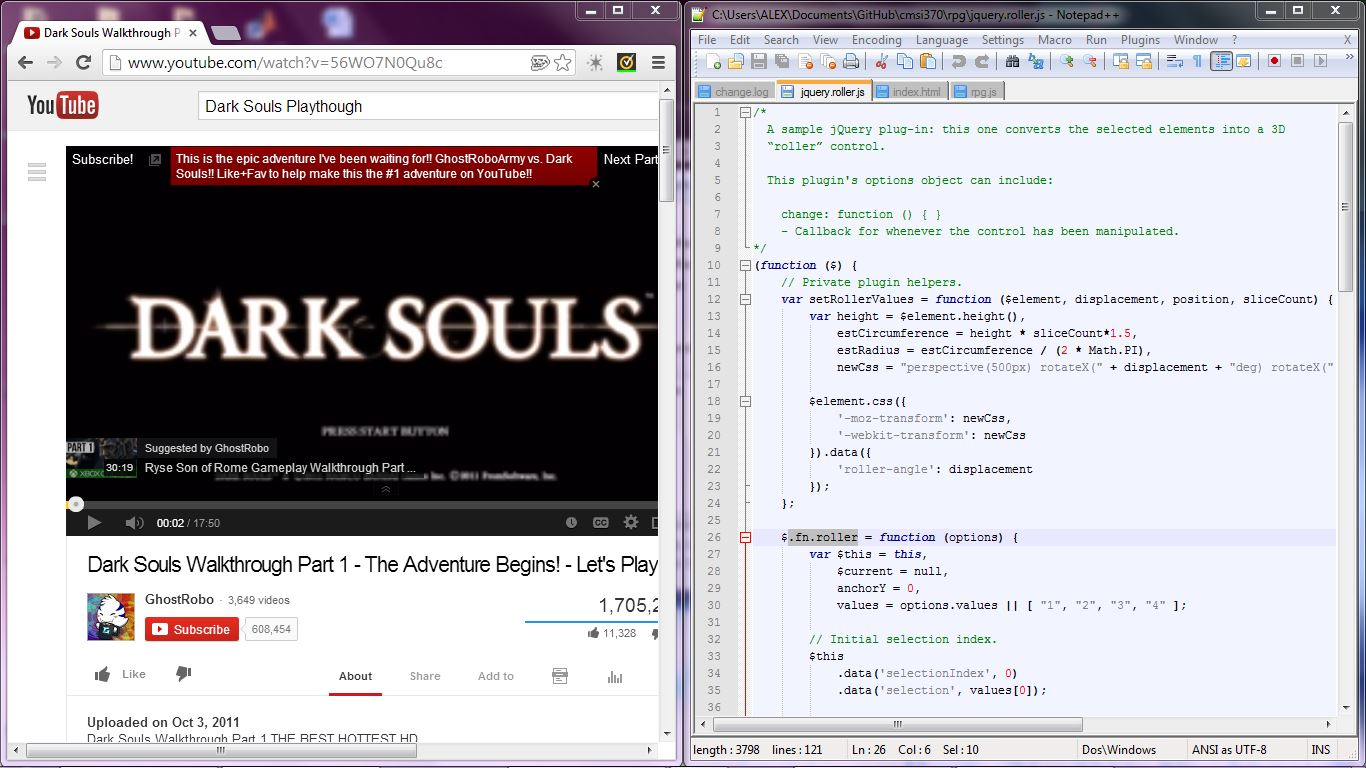
\includegraphics[width= 1\textwidth]{./Images/YoutubeWork}
  \caption{What it is currently like to watch video and do work}
 \label{YouWork}
\end{figure}

\begin{figure}[h!]
 \centering
    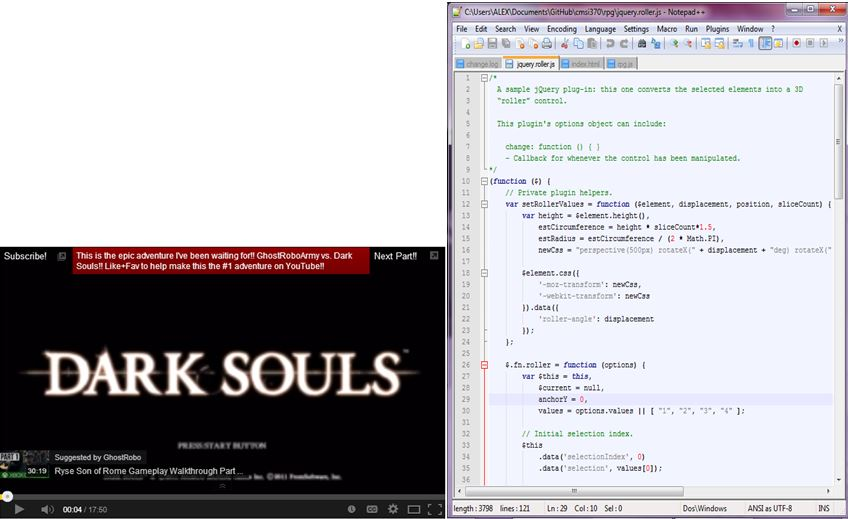
\includegraphics[width= 1\textwidth]{./Images/YoutubeWorkClean}
  \caption{Ideal manner to watch video and do work}
 \label{YouWorkClean}
\end{figure}

\subsection{Internet Security}
Another scenario that makes good use of this browsing system takes advantage of the fact that each brick is an individual browser. This allows for a quick and simple closing of any malicious pop-ups. The individual brick can be immediately shut down without affecting any of the other bricks. This allows for a quick and simple prevention of a possible virus. If this is done behind the scenes and on its own the user will no longer need to be worried by such events. This allows for a less stressful and more enjoyable experience with the internet.
% JD: Many browsers, particularly Chrome, already do this; it's just the format
%     that's different (i.e., tabs vs. bricks).  And again, this is not clearly
%     a user interface element; it has shades of being a new/different feature.
%     We are after the former, not the latter.

\section{Design Rationale}

\subsection{Bricks}
A lot of these ideas come from personal experience and the question, “how can browsing the internet be made more engaging for the user?” The brick idea came about from the idea of direct manipulation. As was stated the idea is to give the user a feel of direct creation, give them the idea that they are the ones responsible for their browsing experience. This allows for the experience to be at the exact level for each person. The size of each brick can be set, but the default will tend to be of moderate size so that the user can clearly see which site is being viewed in a certain brick. As was stated, one of the aspects of web browsing that can’t be avoided is with multiple tabs. The more tabs one is using the more chance for error when attempting to select the desired tab. The use of a brick with an image to represent the contents instead of a title that may not be descriptive at times is a push towards minimizing that error. The biggest inspiration for the brick idea is the appearance of the browser. If the user wants to view the internet in an L shape or in a checkerboard pattern they can do so freely and without much effort. This came from the desire to have a video in YouTube’s full screen mode, but with a smaller window. In this case it is a desire for a full “brick” mode. 
% JD: OK, now *this* clarifies your thinking a little better.  I do happen to
%     agree with you---I think web pages don't give enough flexibility when it
%     comes to presentation of content, particularly videos and sometimes images.
%     I still think that looking up that "web snippet" functionality (and
%     unfortunately I'm not even sure of the name either) might help inform this
%     idea better.

\subsection{Achievements}
The point behind the system of achievements is a subtle push to try and educate more people. It is meant to cause a desire for learning amongst all of the users. As was stated in the video “Doing with Images makes Symbols,” the way programmers have made things has led for complacence amongst the users. The users have all come to accept the level of knowledge they have with their programs and don’t want to make an attempt to learn the system in a deeper level. The idea behind an achievement is to try and get more users to understand their browser and know what it means to be using a browser. These achievements will be made with that in mind and to have people experiment as much as they possibly can. These achievements tend to have some level of desirability on their own, but with social media there is a chance that people will try and do more and learn more than their friends simply due to competitive nature. With everyone pushing one another to greater heights the potential for better browsers, software and interaction design grows. The achievements can have a simple image appear to let the user know they have done well such as the image in Figure  ~\ref{Achieve}. The fact that this browser is so easy to customize and that it will be easy to share, there is a hope for creating a close knit community for the browser. This community will hopefully include all sorts of people ranging from the most serious of programmers to the most humble of internet users.
% JD: OK, so your goal here is to encourage advancement; makes sense, and a good
%     goal.  In that light, perhaps it would be useful not only to post achievements,
%     but also to provide constant feedback toward an achievement.  That way, users
%     will know, even with the smallest of actions, what they got closer to in terms
%     of advancing in knowledge/skill.

\begin{figure}[h!]
 \centering
    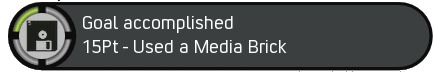
\includegraphics[width= 1\textwidth]{./Images/achievement}
  \caption{Mock Achievement}
 \label{Achieve}
\end{figure}

\subsection{Final Features}
The final group of features is all meant to make the experience better. One of the biggest fears of the older generations when it comes to using the internet is the fear of getting a virus or losing their identity. The internet community often makes fun of this scenario in which newer internet users fall victim to scams that result in them getting a virus. This browser is meant to lower the possibilities of that happening and making the people less fearful of the internet. This will in turn motivate them to explore even more and get them outside of their comfort zone. The idea of the loading screen with timer and something for the user to do is meant to lower possible frustration. For a user, being in the blind and not knowing how much longer one needs to wait to receive the information can be both a waste of time and mentally exhausting. By giving the user a timer of when their webpage will be loaded they are given an indication of how much of their time will not be used on the site, and gives them the opportunity to give up on it if in a hurry, or to do something else while they wait. Essentially the user is being given their time back to do as they please and to be used effectively.
% JD: Yes, I think these motivations were pretty clear even in the earlier section.
%     Which brings me around to another point, related to knowing the difference
%     between a new user interface element vs. a new feature: you interpreted the
%     term "design rationale" as "why I think this idea is good," as opposed to
%     "why this user interface element makes the browser more usable."  It can be
%     subtle, but put it this way: a usability element changes *how* a user does
%     something, but not *what* he or she does.  That's why the bricks idea is
%     clearly usability-related, but the other ideas are less so.
%
%     Another thing that is missing is clarity in whether these ideas are to be
%     taken separately, or integrated into a whole.  The signal I get is "separate."
%     But now, the problem is that is, why put these together?  They now seem forced,
%     just crammed together because of the assignment.  Then again, the assignment is
%     about a dream *interface*, not *interfaces*.  If you are going to list a number
%     of ideas, those ideas should come together into something that makes sense as
%     a unified entity.

\section{Usage Forecast}
The day this browser is first used there will be a lot of getting used to. The hope is that by giving the user the feel of the brick they will automatically see that the tabs are all objects that can be pieced together. However its weak point will come from the fact that the different types of bricks will not be obvious for the users. There will be a good amount of trial and error before it can be used efficiently. This weakness should be lessened somewhat thanks to the achievement system which will let the user know that there are different types of bricks and their uses. These achievements will let the user know without directly telling them and will again add to the sense of self discovery for the users. The high point should be the learnability, satisfaction, and memorability. The achievement system should lead the user to learning how to use this system. The achievements will be made in a step by step manner to get the user to learn it at their own pace. The achievements they unlock will be something that stays with them, even if it was an achievement for which they did the action only once, that memory will stay with them and serve as a constant reminder that such action is possible and is something they have done before. Even if they didn’t quite understand how they did it the first time, they will at least have some sort of idea on how they did it, and can look to the community to help then fill in the missing steps they may have forgotten. The satisfaction should be one of the highest points because the user will always be as satisfied as they want to be. With all of the customization options and the achievements teaching how to customize at will, the users should be using their own dream interface web browser. Overall the browser should be well received by the general public.
% JD: Funny how just as I wrote the previous comment about unification, this last
%     paragraph does finally take a stab at it.  Still, it is just a stab.  For one
%     thing, now you are only talking about bricks and achievement.  What happened
%     to the timing idea?  Or the security/protection feedback?  Even as this paragraph
%     unified bricks and achievements, it quietly acknowledges that timing and security
%     were sort of odd-ones-out.
%
%     One precision point: you talk about learnability in terms of encouraging a user
%     to learn, in relation to achievements.  But remember, learnability is not about
%     encouragement, it is about *speed*.  Don't get me wrong: it's nice to be encouraging
%     and to keep the user engaged.  *But does it make the user figure things out faster?*
%     That point is unaddressed, and its absence misrepresents the meaning of learnability
%     as a usability metric.

\section{Conclusion}
In conclusion this browser should be seen as a beginner’s web browser but also a great tool for developers. It has a full customizability that a beginner can grasp the basics of and a more accustomed user can edit at a much lower level. The brick design is meant to be something familiar to most and communicates the idea of having the ability to be put together. Each brick is meant work on its own and also work with others for a greater brick and different experience. This is what an ideal web browser would be like.
% JD: So, even more interesting now is how your conclusion discusses *only* the brick
%     idea.  This lends even further credence to the impression that the batch of ideas
%     at the beginning do not mesh well together.
%
%     In the end, I think you would have been better off devoting the entire paper to
%     the brick idea, and thinking more deeply about that, right into some of the issues
%     you mention: different types of bricks, how to distinguish them, how they can be
%     manipulated, etc.  The other ideas just get in the way of the bricks.


\end{document}
